\documentclass[11pt,a4paper]{article}

% These are extra packages that you might need for writing the equations:
\usepackage{amsmath}
\usepackage{amsfonts}
\usepackage{amssymb}
\usepackage{booktabs}
\usepackage{hyperref}
\usepackage{listings}
\usepackage{xcolor}
\usepackage{outlines}
\usepackage{mathtools}



\lstset {language=C++,
		 basicstyle=\ttfamily,
         keywordstyle=\color{blue}\ttfamily,
         stringstyle=\color{red}\ttfamily,
         commentstyle=\color{purple}\ttfamily,
         morecomment=[l][\color{magenta}]{\#},
       	 basicstyle=\tiny}

% You need the following package in order to include figures in your report:
\usepackage{graphicx}

% With this package you can set the size of the margins manually:
\usepackage[left=2cm,right=2cm,top=2cm,bottom=2cm]{geometry}

\renewcommand{\vec}[1]{\mathbf{#1}}
\newcommand{\norm}[1]{\left\lVert#1\right\rVert}

\begin{document}

% Enter the exercise number, your name and date here:
\noindent\parbox{\linewidth}{
 \parbox{.25\linewidth}{ \large ICP, Exercise 12 }\hfill
 \parbox{.5\linewidth}{\begin{center} \large Beat Hubmann \end{center}}\hfill
 \parbox{.2\linewidth}{\begin{flushright} \large Dec 07, 2018 \end{flushright}}
}
\noindent\rule{\linewidth}{2pt}


\section{Introduction}

As a continuation of last week's work on exercise 11, the conjugate gradient method was 
implemented to also solve
the discretized Poisson equation in two dimensions for point charges in a grounded box.
This time around, the time to solution was compared to a high performance library Cholesky solver as well 
as to the library Conjugate Gradient solver.

\section{Algorithm Description}

Repeating last week's description:\\
For all cases, the two-dimensional Poisson equation(equation~\ref{eqn:1}) on $\Omega$ is 
discretized using second-order central finite differences in both the x- and the y-direction (equation~\ref{eqn:2}).
Both axes share a common grid spacing of $\Delta x= \frac{1}{N+1}$ where $N$ is the number of interior points
per axis direction on the grid.
Following the established finite difference method procedure to employ natural ordering, the left-hand side of equation~\ref{eqn:2} then can be written
in form of an $N*N \times N*N$ matrix $\vec{A}$ while the values of $\phi$ on the grid get unrolled into a vector $\vec{b}$ of size $N*N$ on the right-hand side (equation~\ref{eqn:3}).\\
The resulting matrix $A$ is both sparse and block tridiagonal.



\begin{equation}
\Delta \Phi = -\phi \quad \text{on}\ \Omega = (0, 1) \times (0,1)
\label{eqn:1}
\end{equation}


\begin{equation}
4x_{i,j} - x_{i-1, j} - x_{x+1, j} - x_{i, j-1} - x_{i, j+1} = -(\Delta x)^2 \cdot \rho(x_{i,j})
\label{eqn:2}
\end{equation}


\begin{equation}
Ax = b
\label{eqn:3}
\end{equation}


\subsection{Conjugate gradient method}
The conjugate gradient method is the most well known member of the family of Krylov subspace methods~\cite{elman}.
Given the system of equations $\vec{Ax}=\vec{b}$ with $\vec{A}$ a symmetric positive definite (SPD) matrix, the method iteratively constructs a solution $\vec{x}^{(t)} \in \mathcal{K}_t(\vec{A}, \vec{r}^{(0)})$ using a starting solution $\vec{x}^{(0)} = (0,0,\ldots, 0)^T$,
the residual $\vec{r}^{(0)}=\vec{b} - \vec{Ax}^{(0)}$ and the associated Krylov subspace $\mathcal{K}_t(\vec{A}, \vec{r}^{(0)})=\text{span}\{\vec{x}, \vec{Ax}, \vec{A}^2\vec{x}, \ldots, \vec{A}^{t-1}\vec{x}\}$.
In this implementation, we use the simple Richardson iteration with $\vec{x}^{(t)}=\vec{x}^{(t-1)} + \alpha_{t-1}\vec{x}^{(t-1)}$ where $\alpha$ is a scalar factor
calculated as shown in the outline below. $\vec{M}^{-1}\ =\ \frac{\delta_{ij}}{\vec{A}_{ii}}$ is the Jacobi preconditioner matrix. Setting $\vec{M} = \vec{M}^{-1} = \vec{\mathcal{I}}$ instead trivially falls back to 
using no preconditioner:
\begin{outline}
\1 $\vec{r}^{(0)} \leftarrow \vec{b} - \vec{Ax}^{(0)}$
\1 $\vec{z}^{(0)} \leftarrow \vec{M}^{-1}\vec{r}^{(0)}$
\1 $\vec{p} \leftarrow \vec{z}^{(0)}$ 
\1 Iterate until convergence and/or iteration limit:
    \2 $\alpha \leftarrow \frac{(\vec{r}^{(t)})^T \vec{z}^{(t)}}{(\vec{p})^T \vec{Ap}}$
    \2 $\vec{x} \leftarrow \vec{x} + \alpha\vec{p}$
    \2 $\vec{r}^{(t)} \leftarrow \vec{r}^{(t-1)} - \alpha\vec{Ap}$
    \2 check preconditioned residual $\norm{\vec{r}^{(t)}}_2$ for convergence; stop if reached
    \2 $\vec{z}^{(t)} \leftarrow \vec{M}^{-1} \vec{r}^{(t-1)}$
    \2 $\beta \leftarrow \frac{(\vec{z}^{(t)})^T \vec{r}^{(t)}}{(\vec{z}^{(t-1)})^T \vec{r}^{(t-1)}}$
    \2 $\vec{p} \leftarrow \vec{z}^{(t)} = \beta \vec{p} $
    \2 $\vec{r}^{(t-1)} \leftarrow \vec{r}^{(t)}$
    \2 $\vec{z}^{(t-1)} \leftarrow \vec{z}^{(t)}$ 
\1 return $\vec{x}$
\end{outline}


\section{Results}

The program was implemented as described above and submitted with this report. \\
The conjugate gradient method was iterated until the residual's norm went below the set treshold: $\norm{\vec{r}}_{2} \le 10^{-4}$.
The conjugate gradient method took only $t=82$ iterations and $\sim 1 \text{ms}$ which compares very favourably with the Jacobi relaxation method ($t=3478$ iterations in $\sim 45 \text{ms}$)
and the Gauss-Seidel method ($t=1922$ iterations in $\sim 6400 \text{ms}$ examined in exercise 11. For comparison, Eigen's optimized library Cholesky method
solver obtained the reference solution in $\sim 10 \text{ms}$ while Eigen's own conjugate gradient method set to use a complete matrix took $\sim 3 \text{ms}$.\\
The conjugate gradient method with the set residual treshold reached a very minor deviation from the reference Cholesky solution:\\ 
$\norm{\vec{x}^*_{\text{Conjugate gradient}} - \vec{x}^*_{\text{Cholesky}}}_{2} \approxeq 0.0002$. \\
The heat map for the conjugate gradient solver is shown in figure~\ref{fig:1}.


\begin{figure}[ht]
\begin{center}
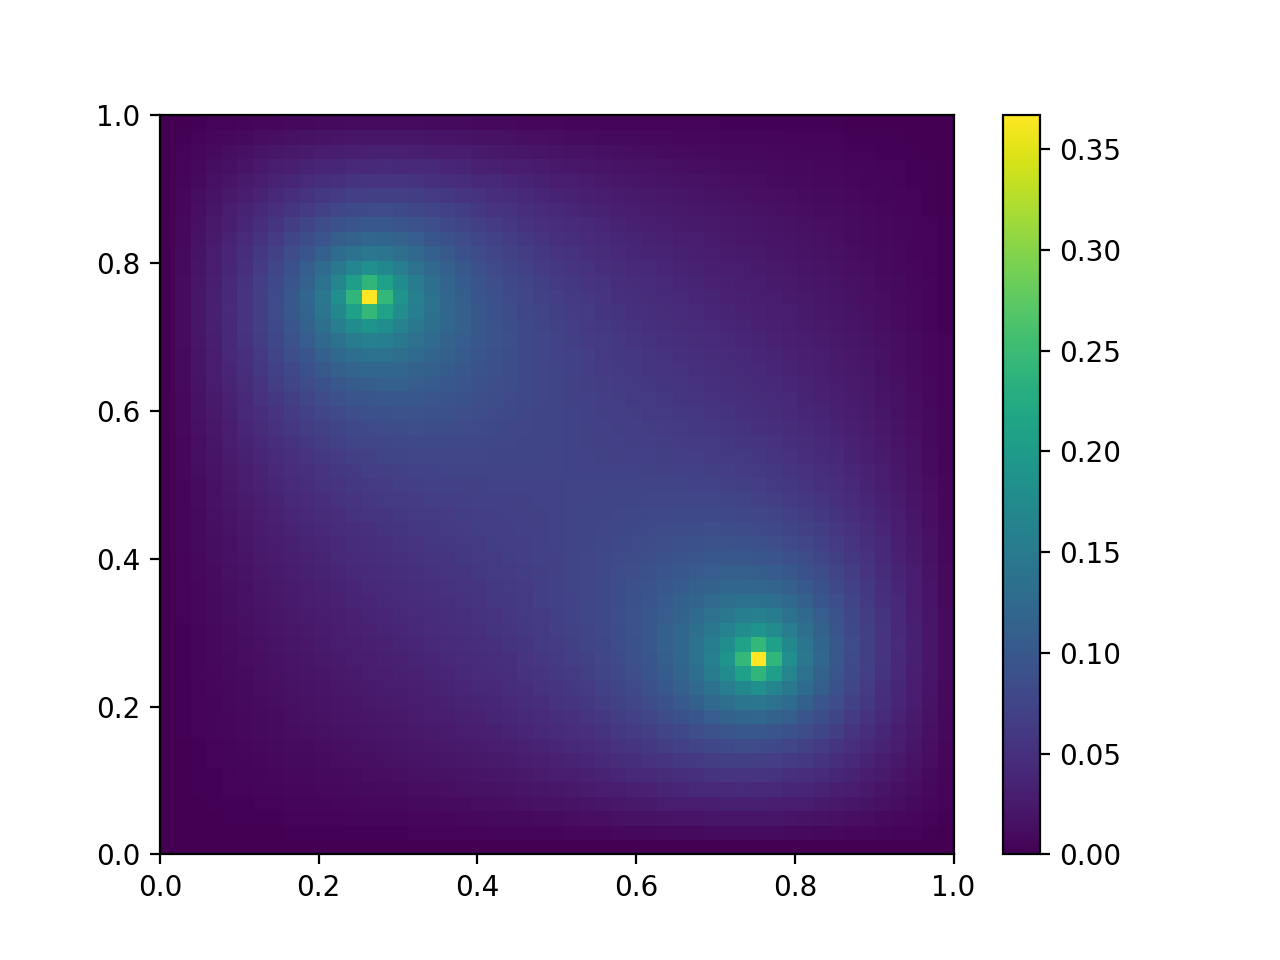
\includegraphics[scale=1.2]{figure_1.png} 
\end{center}
\caption{Conjugate gradient solver reference solution for Poisson equation with point charges at $(0.25, 0.75)$, $(0.75, 0.25)$; grid parameter $N=50$.}
\label{fig:1}
\end{figure}

\section{Discussion}
The results are mostly are as expected, the exception being that the Jacobi preconditioner didn't make a difference for the system under consideration.
Then again, neither is the Jacobi preconditioner sophisticated, nor does the given system setup (2D finite differences on a small system with $N=50$) actually
mandate using a preconditioner.

\begin{thebibliography}{99}


\bibitem{elman}
Elman, H., Silvester, D., Wathen, A. \\
\emph{Finite Elements and Fast Iterative Solvers},\\
Oxford University Press,\\
2014.



% \bibitem{metropolis}
% Metropolis, N.,
% Rosenbluth, A.W.,
% Rosenbluth, M.N.,
% Teller, A.H.,
% Teller, E.\\
% \emph{Equations of State Calculations by Fast Computing Machines},\\
% Journal of Chemical Physics. 21 (6): 1087,\\
% 1953.


% \bibitem{herrmann}
% 	Herrmann, H. J.,
% 	Singer, H. M.,
% 	Mueller L.,
% 	Buchmann, M.-A.,\\
% 	\emph{Introduction to Computational Physics - Lecture Notes},\\
% 	ETH Zurich,\\
% 	2017.

% \bibitem{Gottschling}
% Gottschling, Peter\\
% \emph{Discovering Modern C++},\\
% Addison-Wesley,\\
% 2016.




\end{thebibliography}

\end{document}